% questions.tex —— 2022 年·全国甲卷·理科 · 题目内容片段（无答案）
% 由 tools/generate_projects.py 依来源总账自 2022/2022_数学真题_全国甲理_试题.md 生成，勿手改（改源 MD 后重跑）


\gkpart{数学}

\gkpart{一、单选题}

\begin{question}
\gkti{1}若 $z=-1+\sqrt3\,\mathrm i$，则 $\dfrac{z}{z\overline z-1}=$\mbox{（　　）}

（A）$-1+\sqrt3\,\mathrm i$　　（B）$-1-\sqrt3\,\mathrm i$　　（C）$-\dfrac13+\dfrac{\sqrt3}{3}\,\mathrm i$　　（D）$-\dfrac13-\dfrac{\sqrt3}{3}\,\mathrm i$

\Needspace{0.4\textheight}
\end{question}
\begin{question}
\gkti{2}某社区通过公益讲座以普及社区居民的垃圾分类知识。为了解讲座效果，随机抽取 10 位社区居民，让他们在讲座前和讲座后各回答一份垃圾分类知识问卷，这 10 位社区居民在讲座前和讲座后问卷答题的正确率如下图。图中横轴为居民编号，纵轴为正确率；“*”表示讲座前，“\textbullet{}”表示讲座后。为便于复核图示，按居民编号 1–10 读取的数据如下：

\begin{center}
\begingroup\setlength{\tabcolsep}{4pt}
\begin{tabular}{lrrrrrrrrrr}
\toprule
居民编号 & 1 & 2 & 3 & 4 & 5 & 6 & 7 & 8 & 9 & 10 \\
\midrule
讲座前（*）正确率（\%） & 65 & 60 & 70 & 60 & 65 & 75 & 90 & 85 & 80 & 95 \\
讲座后（\textbullet{}）正确率（\%） & 90 & 85 & 80 & 90 & 85 & 85 & 95 & 100 & 85 & 100 \\
\bottomrule
\end{tabular}
\endgroup
\end{center}

（A）讲座前问卷答题的正确率的中位数小于 70\%  
（B）讲座后问卷答题的正确率的平均数大于 85\%  
（C）讲座前问卷答题的正确率的标准差小于讲座后正确率的标准差  
（D）讲座后问卷答题的正确率的极差大于讲座前正确率的极差
\nopagebreak[4]
\begin{center}\begin{tikzpicture}[x=0.58cm,y=0.13cm]
\draw[->] (0,0) -- (11,0) node[right] {居民编号};
\draw[->] (0,0) -- (0,6.4) node[above] {正确率};
\foreach \x in {1,...,10} {
  \draw (\x,0) -- (\x,0.10) node[below=3pt] {\x};
}
\foreach \v/\y in {60/2.2,65/2.7,70/3.2,75/3.7,80/4.2,85/4.7,90/5.2,95/5.7,100/6.2} {
  \draw[gray!45] (0,\y) -- (10.4,\y);
  \draw (-0.08,\y) -- (0,\y) node[left=3pt] {\v};
}
\node[left=3pt] at (0,0) {0};
\node[rotate=90] at (-0.82,4.3) {（\%）};
\draw[thick] (-0.09,0.62) -- (0.09,0.78);
\draw[thick] (-0.09,0.78) -- (0.09,0.94);
\foreach \x/\y in {1/2.7,2/2.2,3/3.2,4/2.2,5/2.7,6/3.7,7/5.2,8/4.7,9/4.2,10/5.7} {
  \node at (\x,\y) {\scriptsize$*$};
}
\foreach \x/\y in {1/5.2,2/4.7,3/4.2,4/5.2,5/4.7,6/4.7,7/5.7,8/6.2,9/4.7,10/6.2} {
  \fill (\x,\y) circle (2.1pt);
}
\node[anchor=west] at (10.7,5.5) {$*$ 讲座前};
\fill (10.78,4.95) circle (2.1pt);
\node[anchor=west] at (10.98,4.95) {讲座后};
\end{tikzpicture}
\end{center}
\nopagebreak[4]
\end{question}
\begin{question}
\gkti{3}设全集 $U=\{-2,-1,0,1,2,3\}$，集合 $A=\{-1,2\}$，$B=\{x\mid x^2-4x+3=0\}$，则 $\complement_U(A\cup B)=$\mbox{（　　）}

（A）$\{1,3\}$　　（B）$\{0,3\}$　　（C）$\{-2,1\}$　　（D）$\{-2,0\}$

\Needspace{0.4\textheight}
\end{question}
\begin{question}
\gkti{4}如图，网格纸上绘制的是一个多面体的三视图，网格小正方形的边长为 1，则该多面体的体积为\mbox{（　　）}

（A）$8$　　（B）$12$　　（C）$16$　　（D）$20$

三幅投影均画在 $6\times4$ 网格内：左上为梯形轮廓，右上为 $2\times2$ 方形轮廓，下方为 $4\times2$ 矩形轮廓并带中线。
\nopagebreak[4]
\begin{center}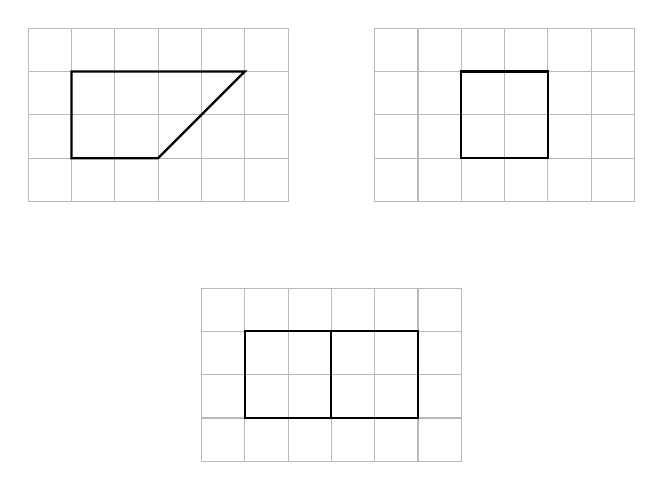
\begin{tikzpicture}[scale=0.55]
\foreach \x/\y in {0/0,8/0,4/-6} {
  \draw[gray!55,thin] (\x,\y) rectangle ++(6,4);
  \foreach \i in {1,...,5} {\draw[gray!55,thin] (\x+\i,\y) -- (\x+\i,\y+4);}
  \foreach \j in {1,2,3} {\draw[gray!55,thin] (\x,\y+\j) -- (\x+6,\y+\j);}
}
\draw[thick] (1,1) -- (3,1) -- (5,3) -- (1,3) -- cycle;
\draw[thick] (10,1) rectangle (12,3);
\draw[thick] (5,-5) rectangle (9,-3);
\draw[thick] (7,-5) -- (7,-3);
\end{tikzpicture}
\end{center}
\nopagebreak[4]
\Needspace{0.4\textheight}
\end{question}
\begin{question}
\gkti{5}函数 $y=(3^x-3^{-x})\cos x$ 在区间 $\left[-\dfrac\pi2,\dfrac\pi2\right]$ 的图象大致为\mbox{（　　）}

（A）–（D）为原卷所示四幅候选曲线图，横轴端点为 $-\pi/2,\pi/2$，纵轴标 $y$。
\nopagebreak[4]
\begin{center}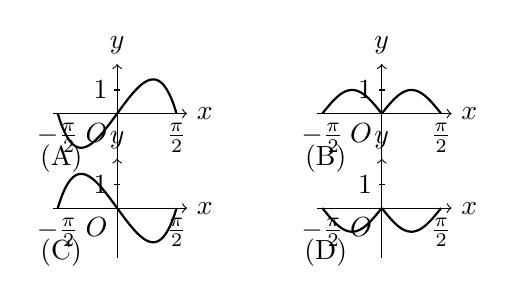
\begin{tikzpicture}[x=0.48cm,y=0.3cm]
\begin{scope}
  \draw[->] (-1.7,0) -- (1.85,0) node[right] {$x$};
  \draw[->] (0,-2.1) -- (0,2.1) node[above] {$y$};
  \draw (-0.08,1) -- (0.08,1);
  \node[below] at (-1.5708,0) {$-\frac\pi2$};
  \node[below] at (1.5708,0) {$\frac\pi2$};
  \node[below left] at (0,0) {$O$};
  \node[left] at (0,1) {$1$};
  \node at (-1.48,-1.9) {(A)};
  \draw[thick,samples=100,domain=-1.5708:1.5708] plot (\x,{(3^(\x)-3^(-1*\x))*cos(deg(\x))});
\end{scope}
\begin{scope}[shift={(7,0)}]
  \draw[->] (-1.7,0) -- (1.85,0) node[right] {$x$};
  \draw[->] (0,-2.1) -- (0,2.1) node[above] {$y$};
  \draw (-0.08,1) -- (0.08,1);
  \node[below] at (-1.5708,0) {$-\frac\pi2$};
  \node[below] at (1.5708,0) {$\frac\pi2$};
  \node[below left] at (0,0) {$O$};
  \node[left] at (0,1) {$1$};
  \node at (-1.48,-1.9) {(B)};
  \draw[thick,samples=100,domain=-1.5708:1.5708] plot (\x,{abs(sin(deg(2*\x)))});
\end{scope}
\begin{scope}[shift={(0,-4)}]
  \draw[->] (-1.7,0) -- (1.85,0) node[right] {$x$};
  \draw[->] (0,-2.1) -- (0,2.1) node[above] {$y$};
  \draw (-0.08,1) -- (0.08,1);
  \node[below] at (-1.5708,0) {$-\frac\pi2$};
  \node[below] at (1.5708,0) {$\frac\pi2$};
  \node[below left] at (0,0) {$O$};
  \node[left] at (0,1) {$1$};
  \node at (-1.48,-1.9) {(C)};
  \draw[thick,samples=100,domain=-1.5708:1.5708] plot (\x,{-(3^(\x)-3^(-1*\x))*cos(deg(\x))});
\end{scope}
\begin{scope}[shift={(7,-4)}]
  \draw[->] (-1.7,0) -- (1.85,0) node[right] {$x$};
  \draw[->] (0,-2.1) -- (0,2.1) node[above] {$y$};
  \draw (-0.08,1) -- (0.08,1);
  \node[below] at (-1.5708,0) {$-\frac\pi2$};
  \node[below] at (1.5708,0) {$\frac\pi2$};
  \node[below left] at (0,0) {$O$};
  \node[left] at (0,1) {$1$};
  \node at (-1.48,-1.9) {(D)};
  \draw[thick,samples=100,domain=-1.5708:1.5708] plot (\x,{-abs(sin(deg(2*\x)))});
\end{scope}
\end{tikzpicture}
\end{center}
\nopagebreak[4]
\end{question}
\begin{question}
\gkti{6}当 $x=1$ 时，函数 $f(x)=a\ln x+\dfrac bx$ 取得最大值 $-2$，则 $f'(2)=$\mbox{（　　）}

（A）$-1$　　（B）$-\dfrac12$　　（C）$\dfrac12$　　（D）$1$

\end{question}
\begin{question}
\gkti{7}在长方体 $ABCD-A_1B_1C_1D_1$ 中，已知 $B_1D$ 与平面 $ABCD$ 和平面 $AA_1B_1B$ 所成的角均为 $30^\circ$，则\mbox{（　　）}

（A）$AB=2AD$  
（B）$AB$ 与平面 $AB_1C_1D$ 所成的角为 $30^\circ$  
（C）$AC=CB_1$  
（D）$B_1D$ 与平面 $BB_1C_1C$ 所成的角为 $45^\circ$

\Needspace{0.4\textheight}
\end{question}
\begin{question}
\gkti{8}沈括的《梦溪笔谈》是中国古代科技史上的杰作，其中收录了计算圆弧长度的“会圆术”。如图，$\widehat{AB}$ 是以 $O$ 为圆心、$OA$ 为半径的圆弧，$C$ 是 $AB$ 的中点，$D$ 在 $\widehat{AB}$ 上，且 $CD\perp AB$。“会圆术”给出 $\widehat{AB}$ 的弧长近似值 $s$ 的计算公式：$s=AB+\dfrac{CD^2}{OA}$。当 $OA=2$，$\angle AOB=60^\circ$ 时，$s=$\mbox{（　　）}

（A）$\dfrac{11-3\sqrt3}{2}$　　（B）$\dfrac{11-4\sqrt3}{2}$　　（C）$\dfrac{9-3\sqrt3}{2}$　　（D）$\dfrac{9-4\sqrt3}{2}$
\nopagebreak[4]
\begin{center}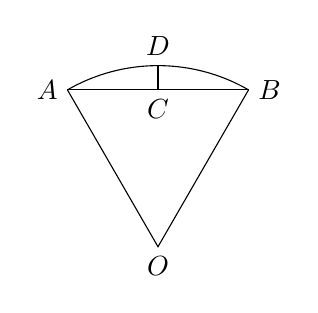
\begin{tikzpicture}[scale=1.15]
\coordinate (O) at (0,-1.732);
\coordinate (A) at (-1,0);
\coordinate (B) at (1,0);
\coordinate (C) at (0,0);
\coordinate (D) at (0,0.268);
\draw (A) -- (O) -- (B);
\draw (A) -- (B);
\draw (O) ++(60:2) arc (60:120:2);
\draw (D) -- (C);
\node[left] at (A) {$A$};
\node[right] at (B) {$B$};
\node[above] at (D) {$D$};
\node[below] at (C) {$C$};
\node[below] at (O) {$O$};
\end{tikzpicture}
\end{center}
\nopagebreak[4]
\end{question}
\begin{question}
\gkti{9}甲、乙两个圆锥的母线长相等，侧面展开图的圆心角之和为 $2\pi$，侧面积分别为 $S_{\text{\text{甲}}}$ 和 $S_{\text{\text{乙}}}$，体积分别为 $V_{\text{\text{甲}}}$ 和 $V_{\text{\text{乙}}}$。若 $\dfrac{S_{\text{\text{甲}}}}{S_{\text{\text{乙}}}}=2$，则 $\dfrac{V_{\text{\text{甲}}}}{V_{\text{\text{乙}}}}=$\mbox{（　　）}

（A）$\sqrt5$　　（B）$2\sqrt2$　　（C）$\sqrt{10}$　　（D）$\dfrac{5\sqrt{10}}4$

\end{question}
\begin{question}
\gkti{10}椭圆 $C:\dfrac{x^2}{a^2}+\dfrac{y^2}{b^2}=1\ (a>b>0)$ 的左顶点为 $A$，点 $P,Q$ 均在 $C$ 上，且关于 $y$ 轴对称。若直线 $AP,AQ$ 的斜率之积为 $\dfrac14$，则 $C$ 的离心率为\mbox{（　　）}

（A）$\dfrac{\sqrt3}{2}$　　（B）$\dfrac{\sqrt2}{2}$　　（C）$\dfrac12$　　（D）$\dfrac13$

\end{question}
\begin{question}
\gkti{11}设函数 $f(x)=\sin\left(\omega x+\dfrac\pi3\right)$ 在区间 $(0,\pi)$ 恰有三个极值点、两个零点，则实数 $\omega$ 的取值范围是\mbox{（　　）}

（A）$\left[\dfrac53,\dfrac{13}6\right)$　　（B）$\left[\dfrac53,\dfrac{19}6\right)$　　（C）$\left(\dfrac{13}6,\dfrac83\right]$　　（D）$\left(\dfrac{13}6,\dfrac{19}6\right]$

\end{question}
\begin{question}
\gkti{12}已知 $a=\dfrac{31}{32}$，$b=\cos\dfrac14$，$c=4\sin\dfrac14$，则\mbox{（　　）}

（A）$c>b>a$　　（B）$b>a>c$　　（C）$a>b>c$　　（D）$a>c>b$

\end{question}
\gkpart{二、填空题}

\begin{question}
\gkti{13}设向量 $\vec a,\vec b$ 的夹角的余弦值为 $\dfrac13$，且 $|\vec a|=1$，$|\vec b|=3$，则 $(2\vec a+\vec b)\cdot\vec b=$\gkblank{}。

\end{question}
\begin{question}
\gkti{14}若双曲线 $y^2-\dfrac{x^2}{m^2}=1\ (m>0)$ 的渐近线与圆 $x^2+y^2-4y+3=0$ 相切，则 $m=$\gkblank{}。

\end{question}
\begin{question}
\gkti{15}从正方体的 8 个顶点中任选 4 个，则这 4 个点在同一个平面的概率为\gkblank{}。

\end{question}
\begin{question}
\gkti{16}已知 $\triangle ABC$ 中，点 $D$ 在边 $BC$ 上，$\angle ADB=120^\circ$，$AD=2$，$CD=2BD$。当 $\dfrac{AC}{AB}$ 取得最小值时，$BD=$\gkblank{}。

\end{question}
\gkpart{三、解答题}

\begin{question}
\gkti{17}记 $S_n$ 为数列 $\{a_n\}$ 的前 $n$ 项和。已知 $\dfrac{2S_n}{n}+n=2a_n+1$。

（1） 证明：$\{a_n\}$ 是等差数列；  
（2） 若 $a_4,a_7,a_9$ 成等比数列，求 $S_n$ 的最小值。

\Needspace{0.4\textheight}
\end{question}
\begin{question}
\gkti{18}在四棱锥 $P-ABCD$ 中，$PD\perp$ 底面 $ABCD$，$CD\parallel AB$，$AD=DC=CB=1$，$AB=2$，$DP=\sqrt3$。

（1） 证明：$BD\perp PA$；  
（2） 求 $PD$ 与平面 $PAB$ 所成的角的正弦值。
\nopagebreak[4]
\begin{center}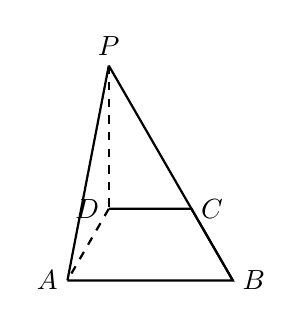
\begin{tikzpicture}[scale=1.05]
\coordinate (A) at (0,0);
\coordinate (B) at (2,0);
\coordinate (C) at (1.5,0.866);
\coordinate (D) at (0.5,0.866);
\coordinate (P) at (0.5,2.598);
\draw[thick] (A)--(B)--(C)--(D);
\draw[thick,dashed] (D)--(A);
\draw[thick] (P)--(A) (P)--(B) (P)--(C);
\draw[thick,dashed] (P)--(D);
\node[left] at (A) {$A$};
\node[right] at (B) {$B$};
\node[right] at (C) {$C$};
\node[left] at (D) {$D$};
\node[above] at (P) {$P$};
\end{tikzpicture}
\end{center}
\nopagebreak[4]
\end{question}
\begin{question}
\gkti{19}甲、乙两个学校进行体育比赛，比赛共设三个项目，每个项目胜方得 10 分，负方得 0 分，没有平局。三个项目比赛结束后，总得分高的学校获得冠军。已知甲学校在三个项目中获胜的概率分别为 $0.5,0.4,0.8$，各项目的比赛结果相互独立。

（1） 求甲学校获得冠军的概率；  
（2） 用 $X$ 表示乙学校的总得分，求 $X$ 的分布列与期望。

\end{question}
\begin{question}
\gkti{20}设抛物线 $C:y^2=2px\ (p>0)$ 的焦点为 $F$，点 $D(p,0)$，过 $F$ 的直线交 $C$ 于 $M,N$ 两点。当直线 $MD$ 垂直于 $x$ 轴时，$|MF|=3$。

（1） 求 $C$ 的方程；  
（2） 设直线 $MD,ND$ 与 $C$ 的另一个交点分别为 $A,B$，记直线 $MN,AB$ 的倾斜角分别为 $\alpha,\beta$。当 $\alpha-\beta$ 取得最大值时，求直线 $AB$ 的方程。

\end{question}
\begin{question}
\gkti{21}已知函数 $f(x)=\dfrac{\mathrm e^x}{x}-\ln x+x-a$。

（1） 若 $f(x)\ge0$，求实数 $a$ 的取值范围；  
（2） 证明：若 $f(x)$ 有两个零点 $x_1,x_2$，则 $x_1x_2<1$。

\end{question}
\begin{question}
\gkti{22}在直角坐标系 $xOy$ 中，曲线 $C_1$ 的参数方程为
\nopagebreak[4]
\[
\begin{cases}
x=\dfrac{2+t}{6},\\
y=\sqrt t
\end{cases}\quad(t\text{ 为参数}),
\]
\Needspace{5\baselineskip}
曲线 $C_2$ 的参数方程为
\nopagebreak[4]
\[
\begin{cases}
x=-\dfrac{2+s}{6},\\
y=-\sqrt s
\end{cases}\quad(s\text{ 为参数}).
\]

（1） 写出 $C_1$ 的普通方程；  
（2） 以坐标原点为极点、$x$ 轴正半轴为极轴建立极坐标系，曲线 $C_3$ 的极坐标方程为 $2\cos\theta-\sin\theta=0$，求 $C_3$ 与 $C_1$ 交点的直角坐标，及 $C_3$ 与 $C_2$ 交点的直角坐标。

\end{question}
\begin{question}
\gkti{23}已知 $a,b,c$ 均为正数，且 $a^2+b^2+4c^2=3$，证明：

（1） $a+b+2c\le3$；  
（2） 若 $b=2c$，则 $\dfrac1a+\dfrac1c\ge3$。

\end{question}